\begin{figure}[H]
	\centering
	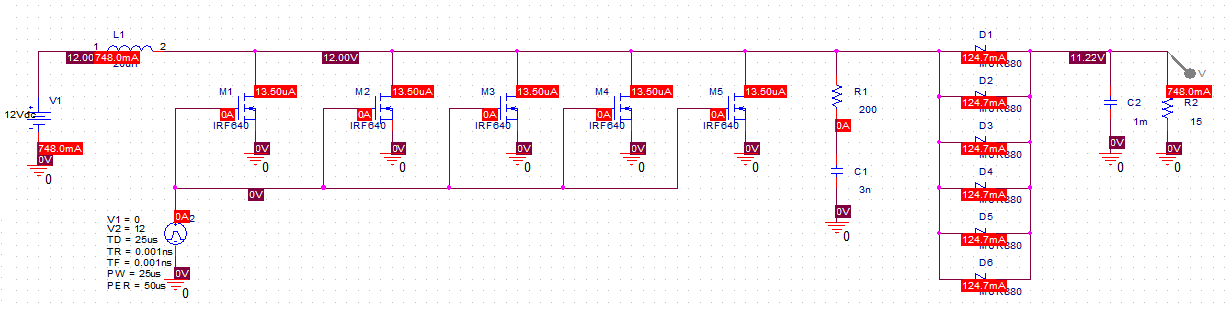
\includegraphics[scale=0.4]{ej2_esq_sim}
	\caption{Simulación en \textit{PSpice}.}
	\label{fig:ej2_esq_sim}
\end{figure}

Se simuló el circuito \ref{fig:ej2_esq_sim}, y se obtuvo la tensión de salida según se ilustra en la Figura \ref{fig:ej2_vo}, aunque posee una pendiente, se puede aproximar $V_S \cong \SI{31}{\volt}$, valor similar al obtenido analíticamente.

\begin{figure}[H]
	\centering
	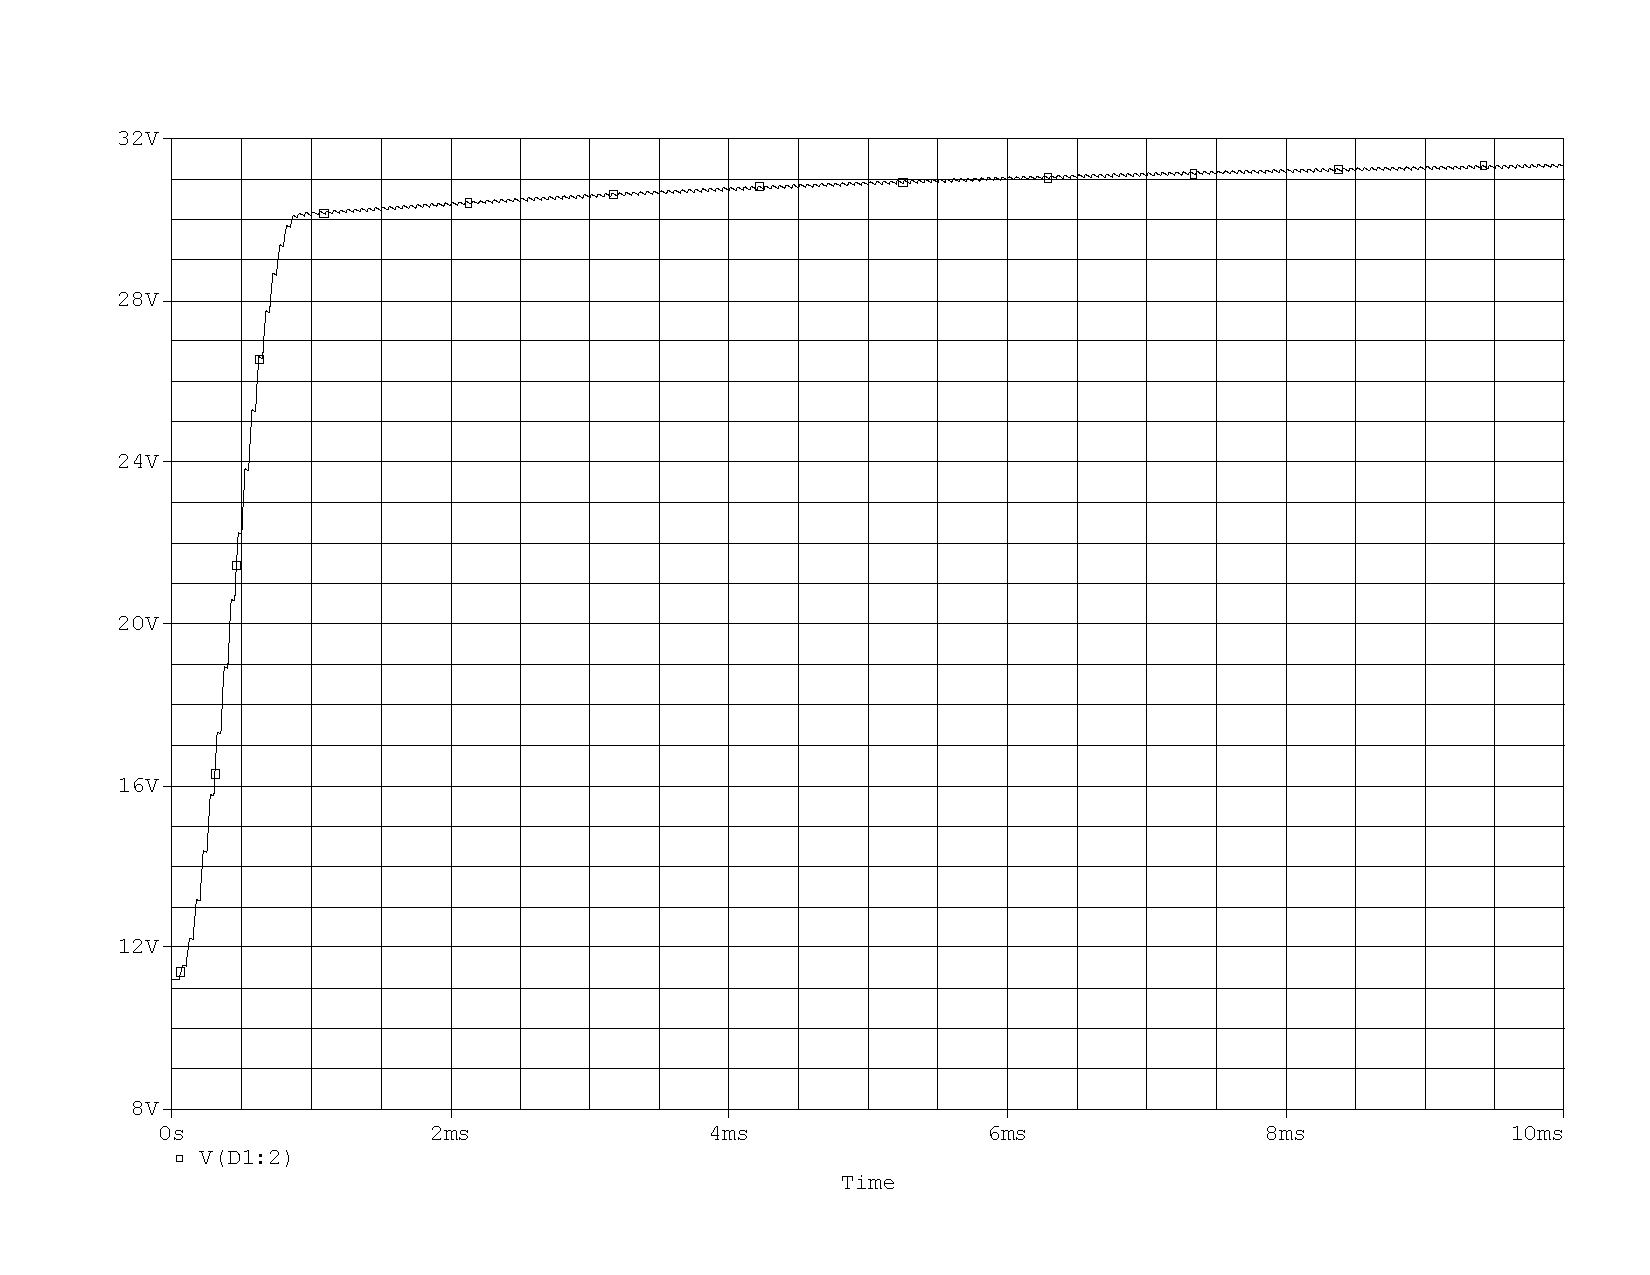
\includegraphics[scale=0.4]{ej2_vo.pdf}
	\caption{Tensión de salida.}
	\label{fig:ej2_vo}
\end{figure}


\begin{figure}[H]
	\centering
	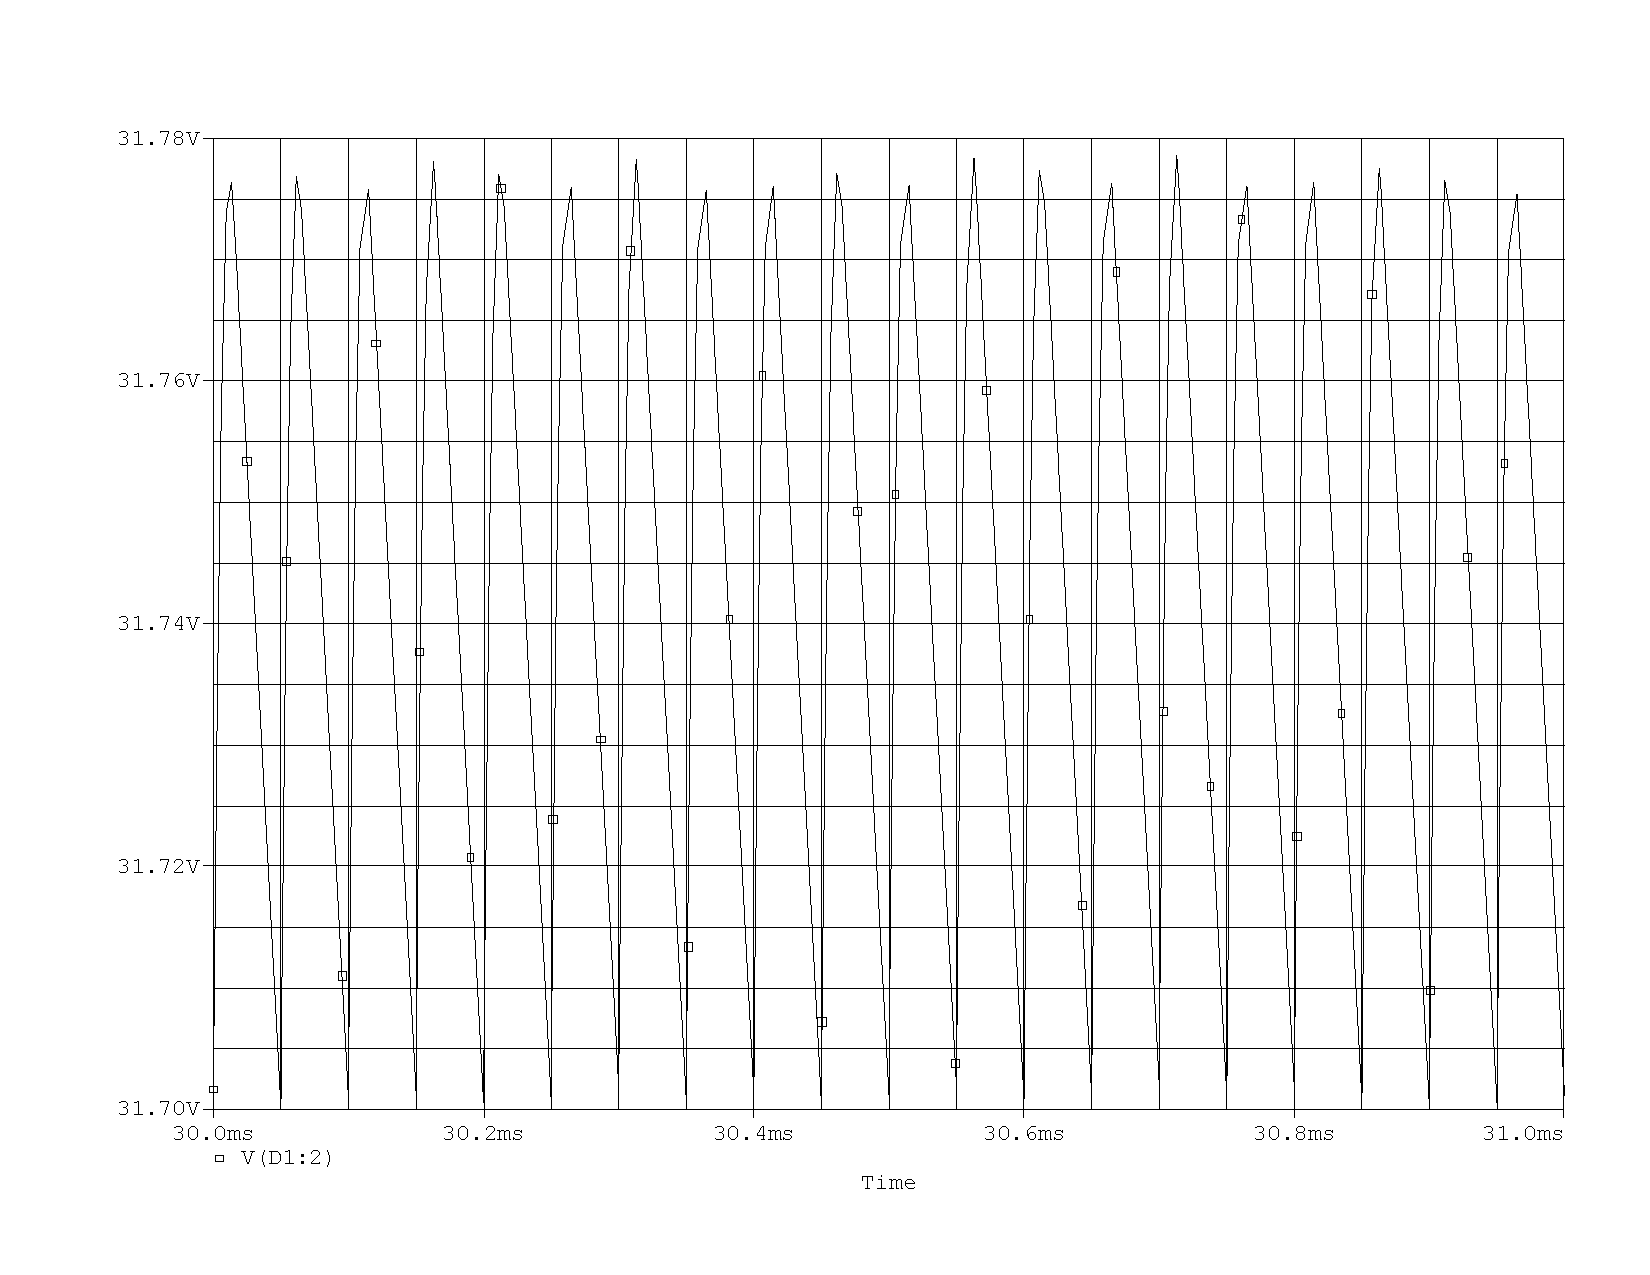
\includegraphics[scale=0.4]{ej2_vo_zoom.pdf}
	\caption{Tensión de salida.}
	\label{fig:ej2_vo_zoom}
\end{figure}

A su vez al ampliar la curva de salida \ref{fig:ej2_vo_zoom} se observa que no es una recta, sino que presenta un rizado de valor \eqref{ec:riz2}.

\begin{equation}
	\centering
	\Delta V_o = \SI{31.775}{\volt} - \SI{31.7}{\volt} = \boxed{\SI{75}{\milli\volt}}
	\label{ec:riz2}
\end{equation}

\begin{figure}[H]
	\centering
	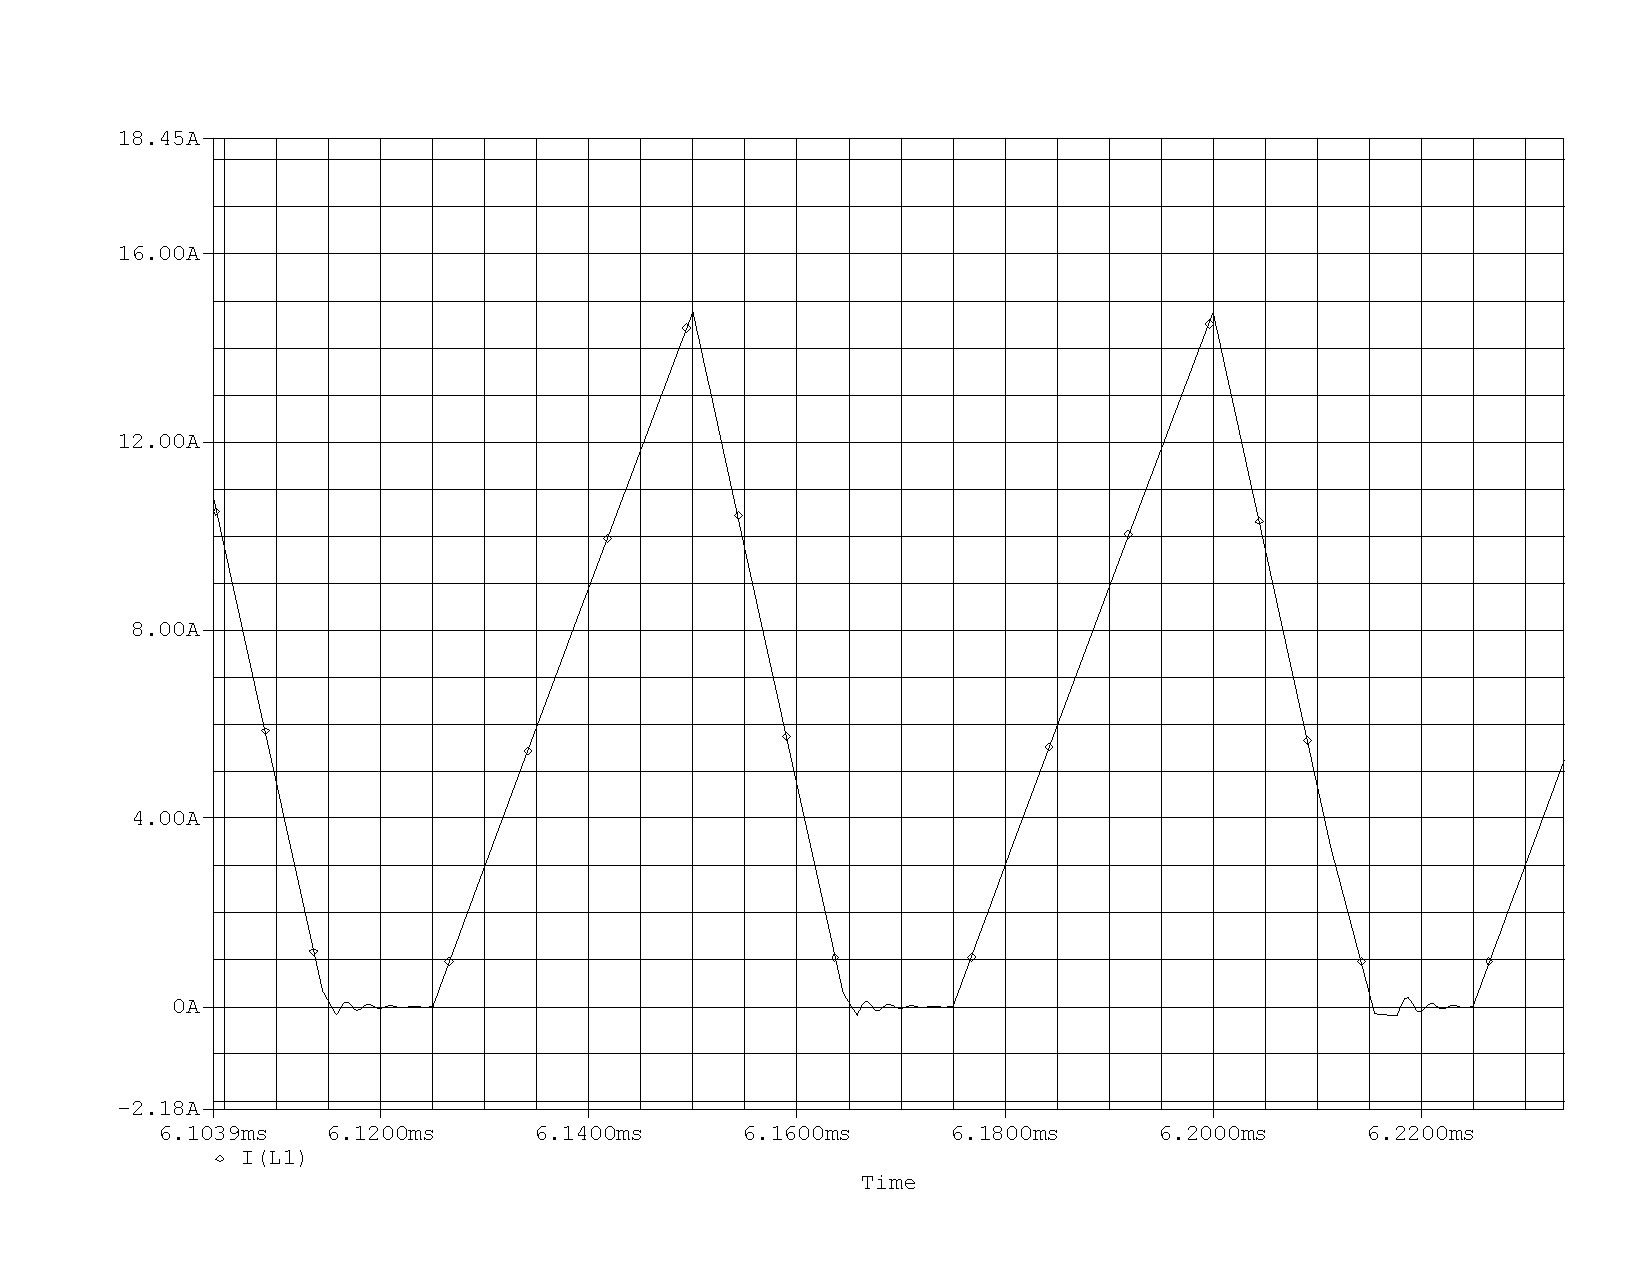
\includegraphics[scale=0.4]{ej2_i_L1.pdf}
	\caption{Corriente en el inductor.}
	\label{fig:ej2_i_L1}
\end{figure}


A partir de la Figura \ref{fig:ej2_i_L1} se verifica el funciomiento del circuito en modo discontinuo, siendo la corriente máxima \SI{14.7}{\ampere} coincidente con la hallada analíticamente. Asimismo se corrobora que el tiempo de carga es mayor que el de descarga, siendo sus valores semejantes a los obtenidos teóricamente.

